\documentclass[t,aspectratio=169,xcolor=dvipsnames]{beamer}

%\usepackage{soul}
\usepackage{multicol}
\usepackage[utf8]{inputenc}
\usepackage{amsmath}
%\usepackage{graphicx}
\usepackage{multirow}
\usepackage{mathtools}
\usepackage[normalem]{ulem} 

% ----------------------------------------------------------------------------------------------------------------------------------------

\title{
\includegraphics[width=45pt]{oepecsetlogo.png}\\(KTXFI2EBNF) Physics II. Supplementary Material}

\author{Dr.~Gábor FACSKÓ, PhD\\\tiny Assistant Professor / Senior Research Fellow\\\textit{facsko.gabor@uni-obuda.hu}}

\institute{\Tiny Óbuda University, Faculty of Electrical Engineering, 1084 Budapest, Tavaszmező u. 17.\\Wigner Research Centre for Physics, Department of Space Physics and Space Technology, 1121 Budapest, Konkoly-Thege Miklós út 29–33.\\ \url{https://wigner.hu/~facsko.gabor}}

\date{December~19,~2025}

\logo{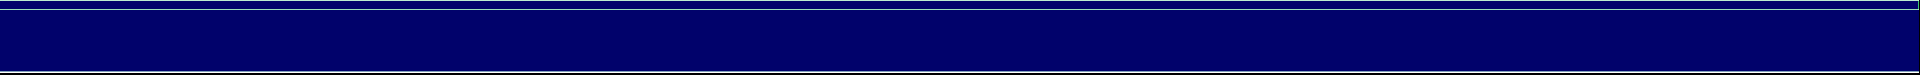
\includegraphics[height=0.9 true cm]{kekcsik.png}}

% ----------------------------------------------------------------------------------------------------------------------------------------

\begin{document}

\frame{\titlepage}

% ----------------------------------------------------------------------------------------------------------------------------------------

\begin{frame}[fragile,squeeze,allowframebreaks]
\frametitle{Justifying of this Material}
\begin{itemize}
\setlength{\parskip}{0pt}
\setlength{\itemsep}{0pt}
\item We did not have sufficient time to cover the following topics:
\begin{itemize}
  \item Basic concepts of nuclear physics.
  \item Basic concepts of particle physics.
\end{itemize}
\item I can only briefly outline what these topics encompass: radioactivity, isotopes, neutron radiation, radiation protection, neutron-induced nuclear fission, thermonuclear fusion, nuclear batteries, types of nuclear reactors, thermonuclear experiments, nuclear weapons, thermonuclear weapons, nuclear waste management, the Hungarian Nuclear Power Plant in Paks, and future technologies such as advanced reactors, high-temperature reactors, thorium reactors, and modular reactors.
\item What could I meaningfully tell you about particle physics at this point? For example: hadrons, mesons, leptons, quarks, or particle colliders?
\pagebreak
\item We have run out of time; therefore, I will send you additional links, or I may record and upload a short personal video exclusively for you.

\item Naturally, none of these topics will be included in the midterm or final examinations.
\end{itemize}
\end{frame}

% ----------------------------------------------------------------------------------------------------------------------------------------

\begin{frame}[fragile,squeeze,allowframebreaks]
\frametitle{Basic concepts of nuclear physics}
\begin{itemize}
\setlength{\parskip}{0pt}
\setlength{\itemsep}{0pt}
\item Radioactivity, isotopes, neutron radiation, radiation protection:
  \begin{itemize}
  \item \href{https://www.cea.fr/english/Documents/thematic-publications/radioactivity.pdf}{Radioactivity}
  \item \href{https://atomeromu.mvm.hu/en/Tudastar/HogyanMukodik}{Nuclear Power Plant in Paks}
  \item \href{https://en.wikipedia.org/wiki/Neutron_radiation}{Neutron Radiation}
  \item \href{https://en.wikipedia.org/wiki/Radiation_protection}{Radiation Protection}
\end{itemize}
\item Neutron-induced nuclear fission, thermonuclear fusion, nuclear batteries, types of nuclear reactors, thermonuclear experiments, nuclear weapons, thermonuclear weapons, nuclear waste management:
  \begin{itemize}
  \item \href{https://www.atomicarchive.com/science/fission/chain-reactions.html}{Chain Reaction}
  \item \href{https://world-nuclear.org/information-library/current-and-future-generation/nuclear-fusion-power}{Nuclear Fusion Experiments}
  \item \href{https://www.britannica.com/science/nuclear-fusion/Fusion-reactions-in-stars}{Stellar Nuclear Fusion}
  \item \href{https://www.researchgate.net/publication/242879324_The_last_natural_nuclear_fission_reactor}{Natural Fission Reactor}
  \item \href{https://www.britannica.com/technology/nuclear-weapon}{Nuclear Weapons}
  \item \href{https://science.nasa.gov/planetary-science/programs/radioisotope-power-systems/overview/}{Radioisotope Thermoelectric Generator (RTG)}

  \pagebreak
  \item \href{https://world-nuclear.org/information-library/nuclear-fuel-cycle/nuclear-waste/radioactive-waste-management}{Radioactive Waste Management}
  \item \href{https://www.imdb.com/title/tt15398776/}{Oppenheimer}
  \item \href{https://www.imdb.com/title/tt0057012/}{Dr. Strangelove or: How I Learned to Stop Worrying and Love the Bomb}
  \end{itemize}
  
\item Future technologies such as advanced reactors, high-temperature reactors, thorium reactors, and modular reactors:
  \begin{itemize}
  \item \href{https://world-nuclear.org/information-library/nuclear-power-reactors/other/advanced-nuclear-power-reactors}{Advanced Nuclear Reactors}
  \item \href{https://world-nuclear.org/information-library/current-and-future-generation/thorium}{Thorium Reactors}
  \item \href{https://world-nuclear.org/information-library/nuclear-power-reactors/small-modular-reactors/small-modular-reactors}{Small Modular Reactors}
  \end{itemize}
\end{itemize}
\end{frame}

% ----------------------------------------------------------------------------------------------------------------------------------------

\begin{frame}%[fragile,squeeze,allowframebreaks]
\frametitle{Basic concepts of particle physics}
\begin{itemize}
\setlength{\parskip}{0pt}
\setlength{\itemsep}{0pt}
\item \href{https://www.britannica.com/science/standard-model}{Hadrons, Mesons, Leptons, Quarks}
\item \href{https://home.cern/}{Conseil Européen pour la Recherche Nucléaire (CERN)}
\end{itemize}
\end{frame}

% ----------------------------------------------------------------------------------------------------------------------------------------

\begin{frame}
%\frametitle{Minden jó, ha a vége jó}

\vfill
\begin{center}
\textbf{\huge The End}

\bigskip
Thank you for your attention!
\end{center}
\vfill
\end{frame}

\end{document}


\documentclass[t,aspectratio=169,xcolor=dvipsnames]{beamer}

%\usepackage{soul}
\usepackage{multicol}
\usepackage[utf8]{inputenc}
\usepackage{amsmath}
%\usepackage{graphicx}
\usepackage{multirow}
\usepackage{mathtools}
\usepackage[normalem]{ulem} 

% ----------------------------------------------------------------------------------------------------------------------------------------

\title{
\includegraphics[width=45pt]{oepecsetlogo.png}\\(KTXFI2EBNF) Physics II. Lecture}

\author{Dr.~Gábor FACSKÓ, PhD\\\tiny Assistant Professor / Senior Research Fellow\\\textit{facsko.gabor@uni-obuda.hu}}

\institute{\Tiny Óbuda University, Faculty of Electrical Engineering, 1084 Budapest, Tavaszmező u. 17.\\Wigner Research Centre for Physics, Department of Space Physics and Space Technology, 1121 Budapest, Konkoly-Thege Miklós út 29–33.\\ \url{https://wigner.hu/~facsko.gabor}}

\date{December~18,~2025}

\logo{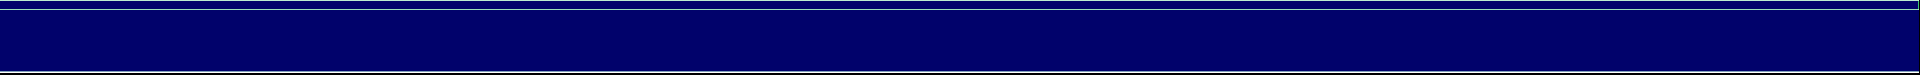
\includegraphics[height=0.9 true cm]{kekcsik.png}}

% ----------------------------------------------------------------------------------------------------------------------------------------

\begin{document}

\frame{\titlepage}

% ----------------------------------------------------------------------------------------------------------------------------------------

\begin{frame}[fragile,squeeze,allowframebreaks]
\frametitle{Common Business}
\begin{itemize}
\setlength{\parskip}{0pt}
\setlength{\itemsep}{0pt}
\item We did not have sufficient time to cover the following topics:
\begin{itemize}
  \item Basic concepts of nuclear physics.
  \item Basic concepts of particle physics.
\end{itemize}
\item I can only briefly outline what these topics include: radioactivity, isotopes, neutron radiation, radiation protection, neutron-induced nuclear fission, thermonuclear fusion, nuclear batteries, types of nuclear reactors, thermonuclear experiments, nuclear weapons, thermonuclear weapons, management of nuclear waste, the Hungarian Nuclear Power Plant in Paks, and future technologies such as advanced reactors, high-temperature reactors, thorium reactors, and modular reactors.
\item What could I meaningfully tell you about particle physics at this point? For example: hadrons, mesons, leptons, quarks, or particle colliders?
\item We are out of time; therefore, I will send you additional links, or I may record and upload a short personal video exclusively for you.

\pagebreak
\item Naturally, none of these topics will be included in the midterm or final examinations.
\end{itemize}
\end{frame}

% ----------------------------------------------------------------------------------------------------------------------------------------

\begin{frame}[fragile,squeeze,allowframebreaks]
\frametitle{Basic concepts of nuclear physics}
\begin{itemize}
\setlength{\parskip}{0pt}
\setlength{\itemsep}{0pt}
\item Radioactivity, isotopes, neutron radiation, radiation protection:
  \begin{itemize}
  \item \href{https://www.cea.fr/english/Documents/thematic-publications/radioactivity.pdf}{Radioactivity}
  \item  \href{https://atomeromu.mvm.hu/en/Tudastar/HogyanMukodik}{Nuclear Powerplant in Paks}
  \item \href{https://en.wikipedia.org/wiki/Neutron_radiation}{Neutron Radiation}
    \item \href{https://en.wikipedia.org/wiki/Radiation_protection}{Radiation Projection}
\end{itemize}
\item Neutron-induced nuclear fission, thermonuclear fusion, nuclear batteries, types of nuclear reactors, thermonuclear experiments,nuclear weapons, thermonuclear weapons, management of nuclear waste:
  \begin{itemize}
  \item \href{https://www.atomicarchive.com/science/fission/chain-reactions.html}{Chain Reaction}
  \item \href{https://world-nuclear.org/information-library/current-and-future-generation/nuclear-fusion-power}{Nuclear Fusion Experiments}
  \item \href{https://www.britannica.com/science/nuclear-fusion/Fusion-reactions-in-stars}{Stellar Nuclear Fusion}
  \item \href{https://www.researchgate.net/publication/242879324_The_last_natural_nuclear_fission_reactor}{Natural Fission Reactor}
  \item \href{https://www.britannica.com/technology/nuclear-weapon}{Nuclear Weapons}
  \item \href{https://science.nasa.gov/planetary-science/programs/radioisotope-power-systems/overview/}{Radioisotope Thermoelectric Generator (RTG)}

  \pagebreak
  \item \href{https://world-nuclear.org/information-library/nuclear-fuel-cycle/nuclear-waste/radioactive-waste-management}{Radioactive Waster Management}
  \item \href{https://www.imdb.com/title/tt15398776/}{Oppenheimer}
  \item \href{https://www.imdb.com/title/tt0057012/}{Dr. Strangelove or: How I Learned to Stop Worrying and Love the Bomb}
  \end{itemize}
  
\item Future technologies such as advanced reactors, high-temperature reactors, thorium reactors, and modular reactors:

  \begin{itemize}
  \item \href{https://world-nuclear.org/information-library/nuclear-power-reactors/other/advanced-nuclear-power-reactors}{Advanced Nuclear Reactors}
  \item \href{https://world-nuclear.org/information-library/current-and-future-generation/thorium}{Thorium Reactors}
  \item \href{https://world-nuclear.org/information-library/nuclear-power-reactors/small-modular-reactors/small-modular-reactors}{Small Modular Reactors}
  \end{itemize}
\end{itemize}
\end{frame}

% ----------------------------------------------------------------------------------------------------------------------------------------

\begin{frame}[fragile,squeeze,allowframebreaks]
\frametitle{Basic concepts of particle physics}
\begin{itemize}
\setlength{\parskip}{0pt}
\setlength{\itemsep}{0pt}
\item \href{https://www.britannica.com/science/standard-model}{Hadrons, Mesons, Leptons, Quarks}
\item \href{https://home.cern/}{Conseil Européen pour la Recherche Nucléaire (CERN)}
  
\end{itemize}
\end{frame}

% ----------------------------------------------------------------------------------------------------------------------------------------

\begin{frame}
%\frametitle{Minden jó, ha a vége jó}

\vfill
\begin{center}
\textbf{\huge The End}

\bigskip
Thank you for your attention!
\end{center}
\vfill
\end{frame}

\end{document}
